\section{Analysis and Simulation: Sampling and Frequency Analysis}
\begin{frame}[t,allowframebreaks]{Table of contents}
\tableofcontents[currentsection,hidesubsections]
\end{frame}


\subsection{Aliasing}
\begin{frame}[t,allowframebreaks]{Sampling a Cos wave and Aliasing Frequency}

\begin{figure}[ht]
\centering
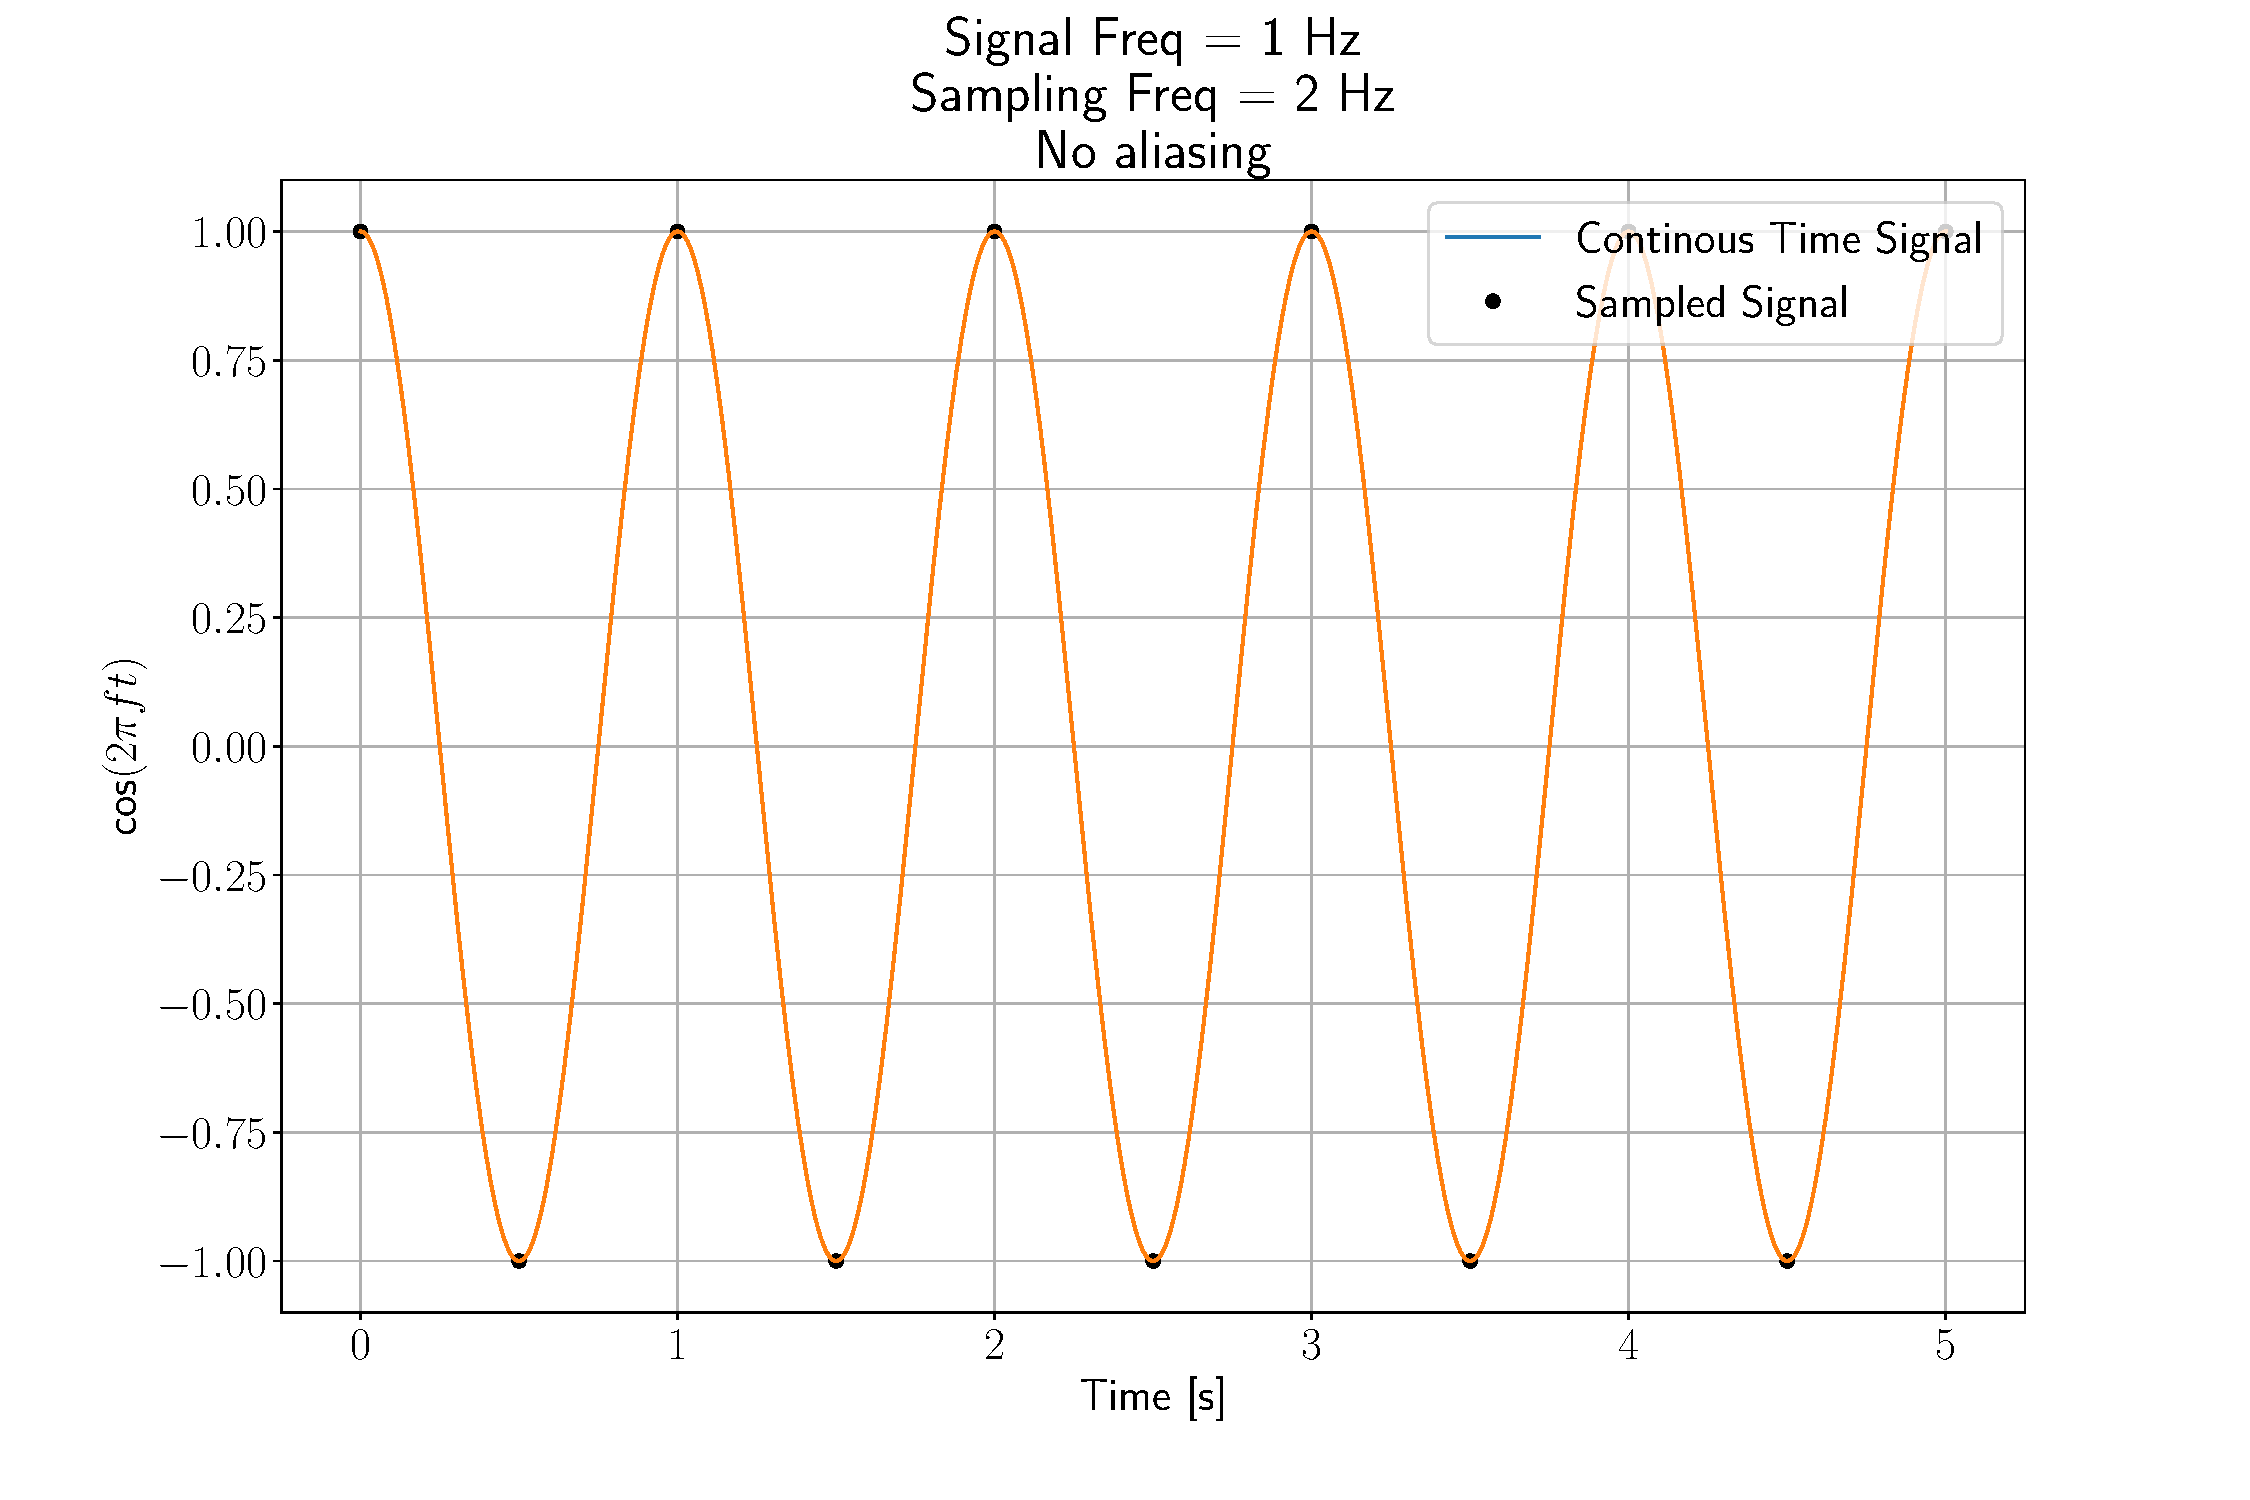
\includegraphics[width = 0.6\textwidth]{Figures/Simulation_Sampling_Frequency_Analysis/Signal_No_Alias_0}
\caption{Sampling at Nyquist Rate: No Aliasing occur}
\label{fig:Simulation_Sampling_Frequency_Analysis:Signal_No_Alias_0}
\end{figure}

\begin{itemize}

\item The signal is from 1 to 5s with a time step of 1ms.

\end{itemize}

\newpage
\begin{figure}[ht]
\centering
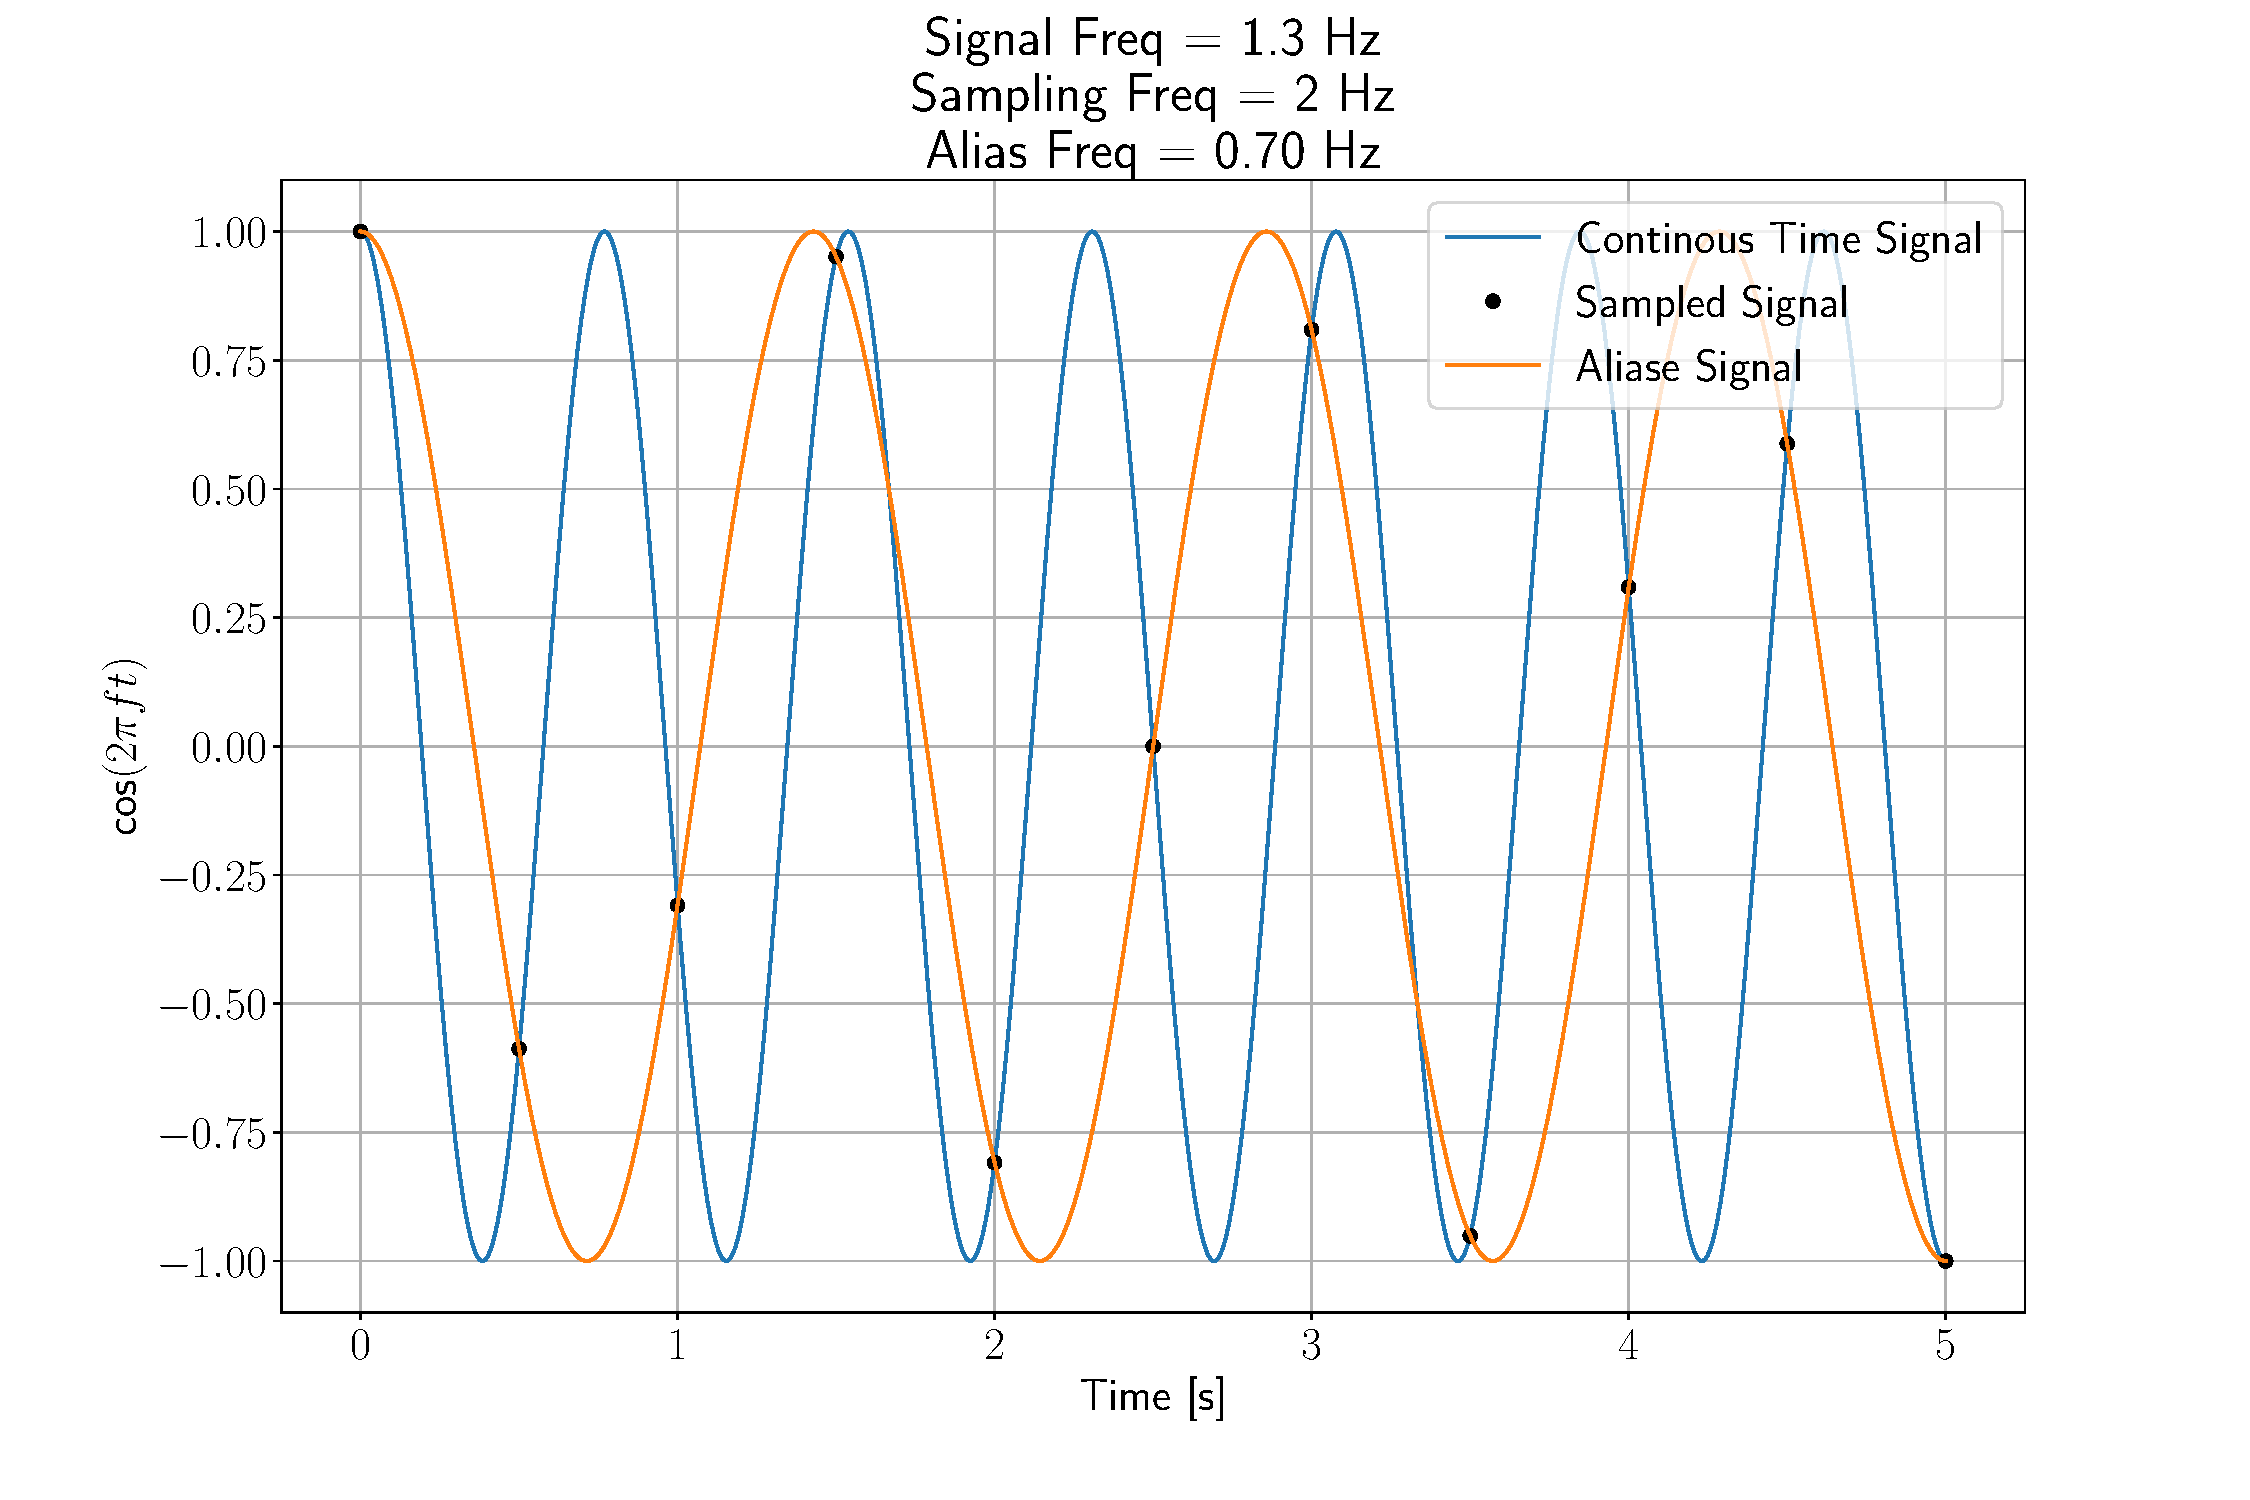
\includegraphics[width = 0.6\textwidth]{Figures/Simulation_Sampling_Frequency_Analysis/Signal_Alias_0_70}
\caption{Increasing Signal Frequency}
\label{fig:Simulation_Sampling_Frequency_Analysis:Signal_Alias_0_70}
\end{figure}

\begin{itemize}

\item Signal frequency is increased and Nyquist rate is not respected now

	\begin{itemize}
	\item $F_s \, < \, 2 \, f_{\text{signal}}$
	\end{itemize}

\item As a result aliasing occur at $f_{\text{alias}} \, = \, 0.7 $ Hz

\end{itemize}


\newpage
\begin{figure}[ht]
\centering
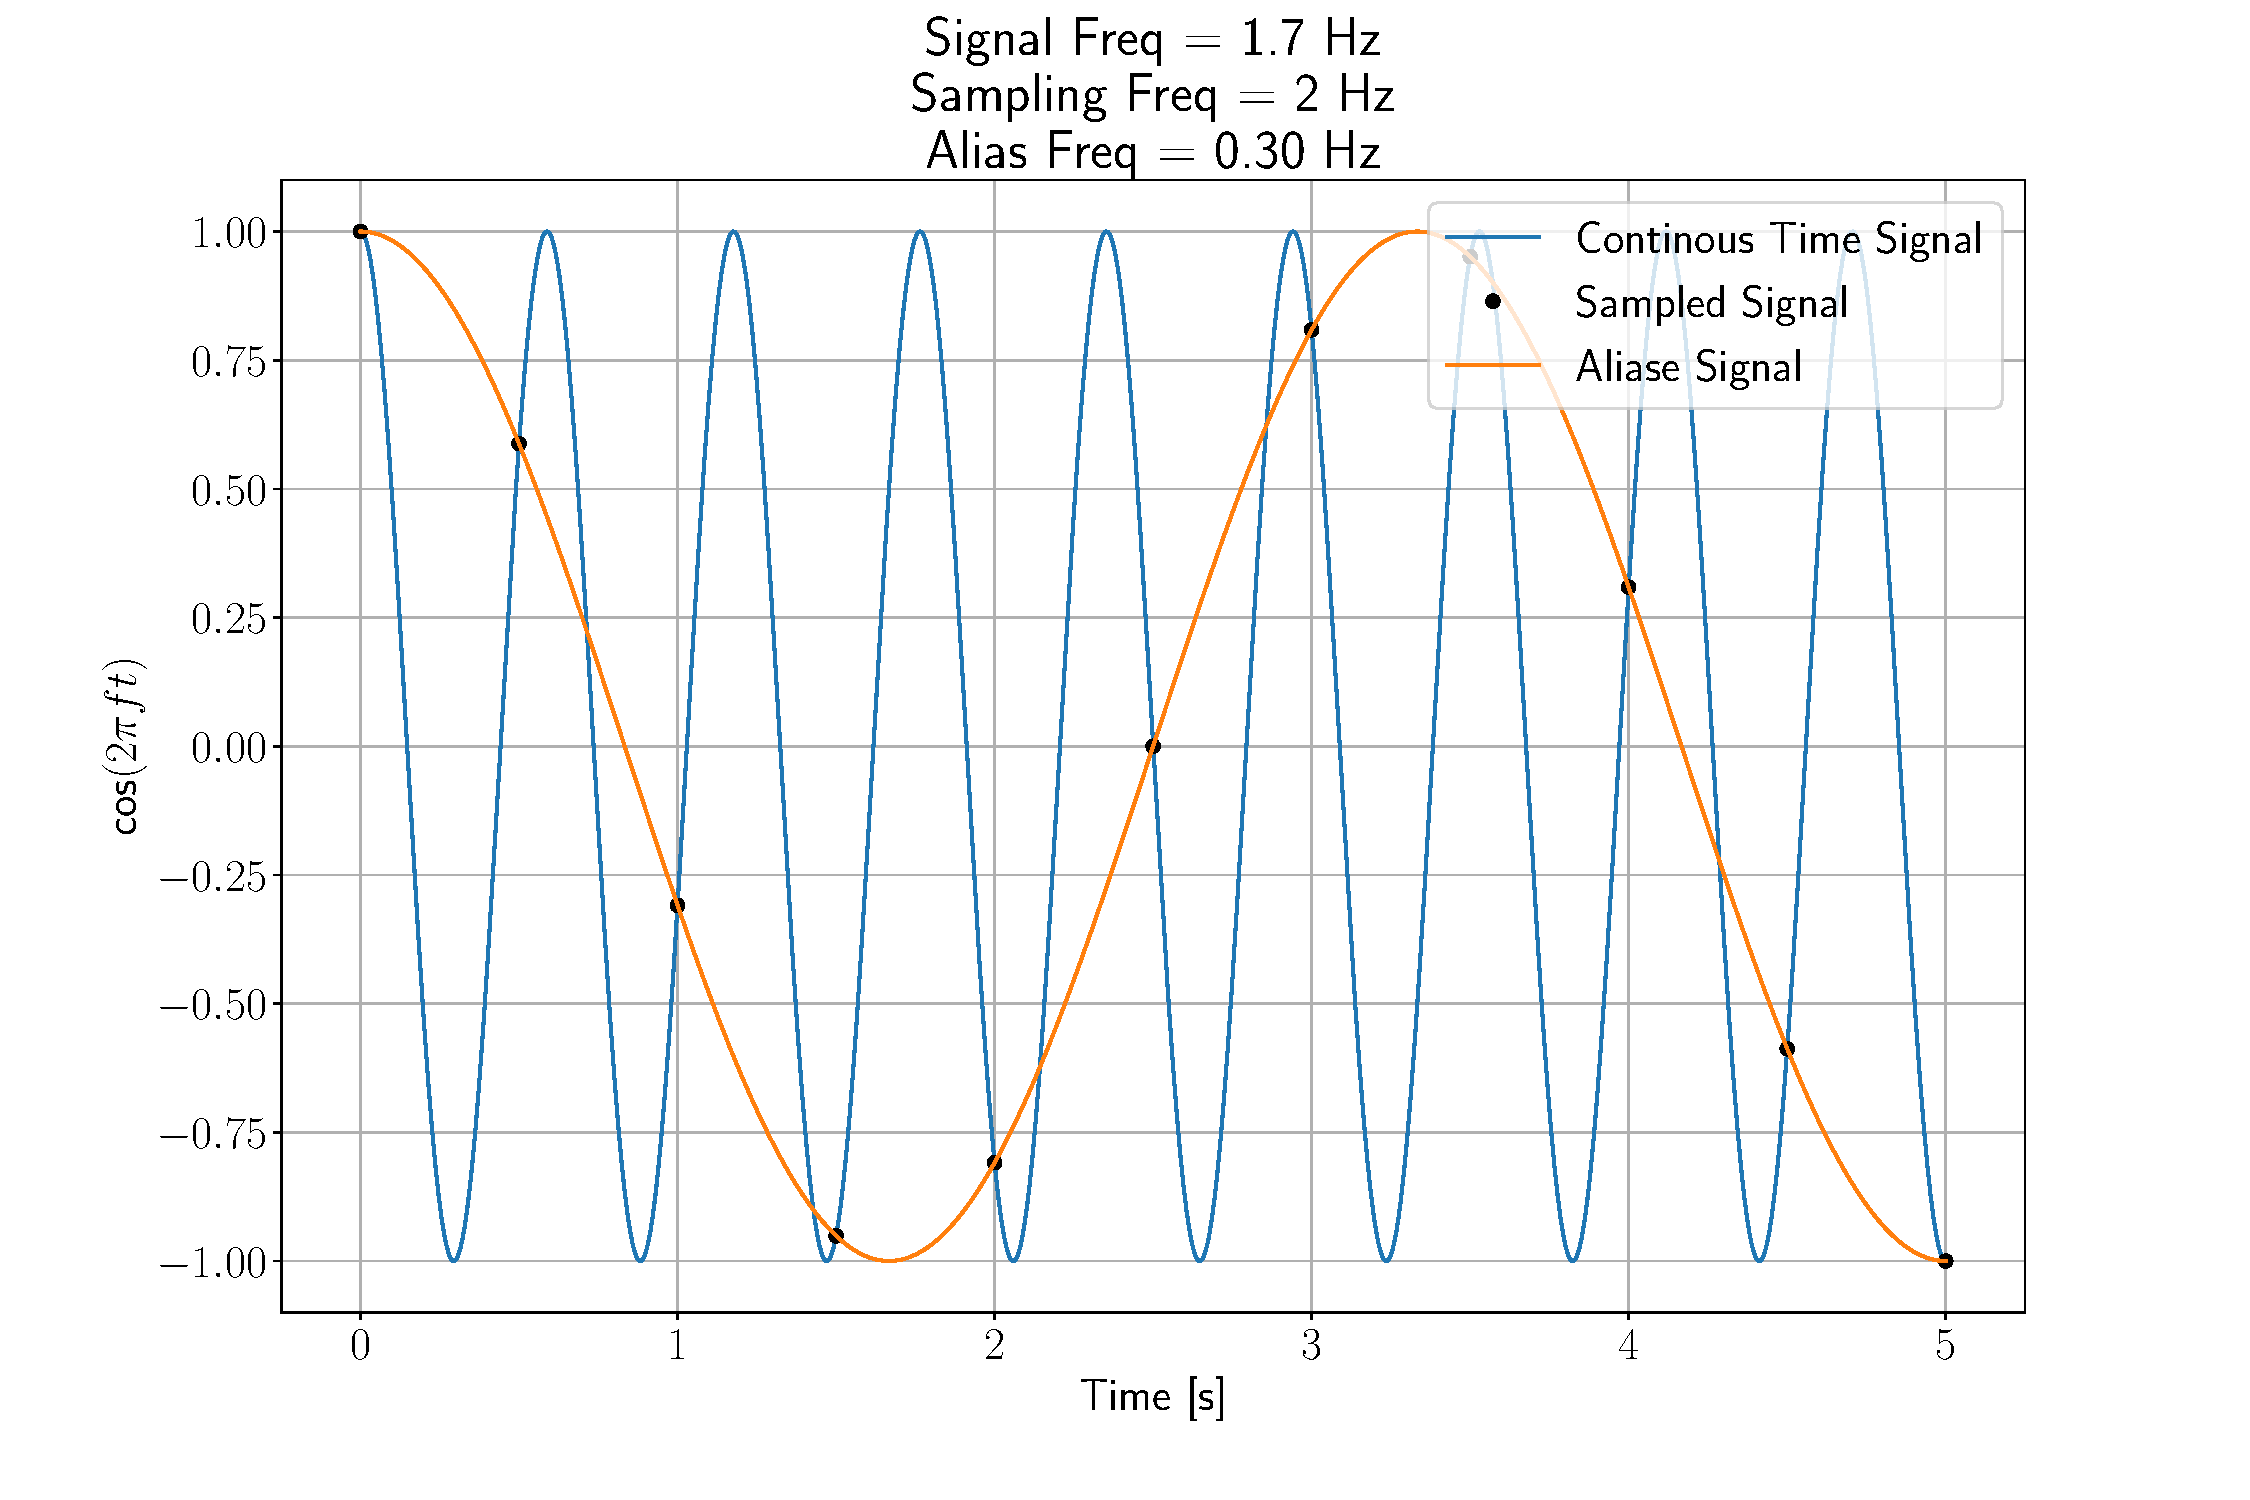
\includegraphics[width = 0.6\textwidth]{Figures/Simulation_Sampling_Frequency_Analysis/Signal_Alias_0_30}
\caption{Sampling at Nyquist Rate: No Aliasing occur}
\label{fig:Simulation_Sampling_Frequency_Analysis:Signal_Alias_0_30}
\end{figure}


\begin{itemize}

\item The signal frequency is even more lower

\item The more we get to the Nyquist rate, the lower $f_{\text{alias}}$ is

	\begin{itemize}
	\item We fail to capture signal information (here frequency content)
	\end{itemize}

\end{itemize}

\end{frame}




\subsection{Zero Padding on FFT for CTFT}
\begin{frame}[t,allowframebreaks]{Zero Padding for the CTFT}

\begin{figure}[ht]
\centering
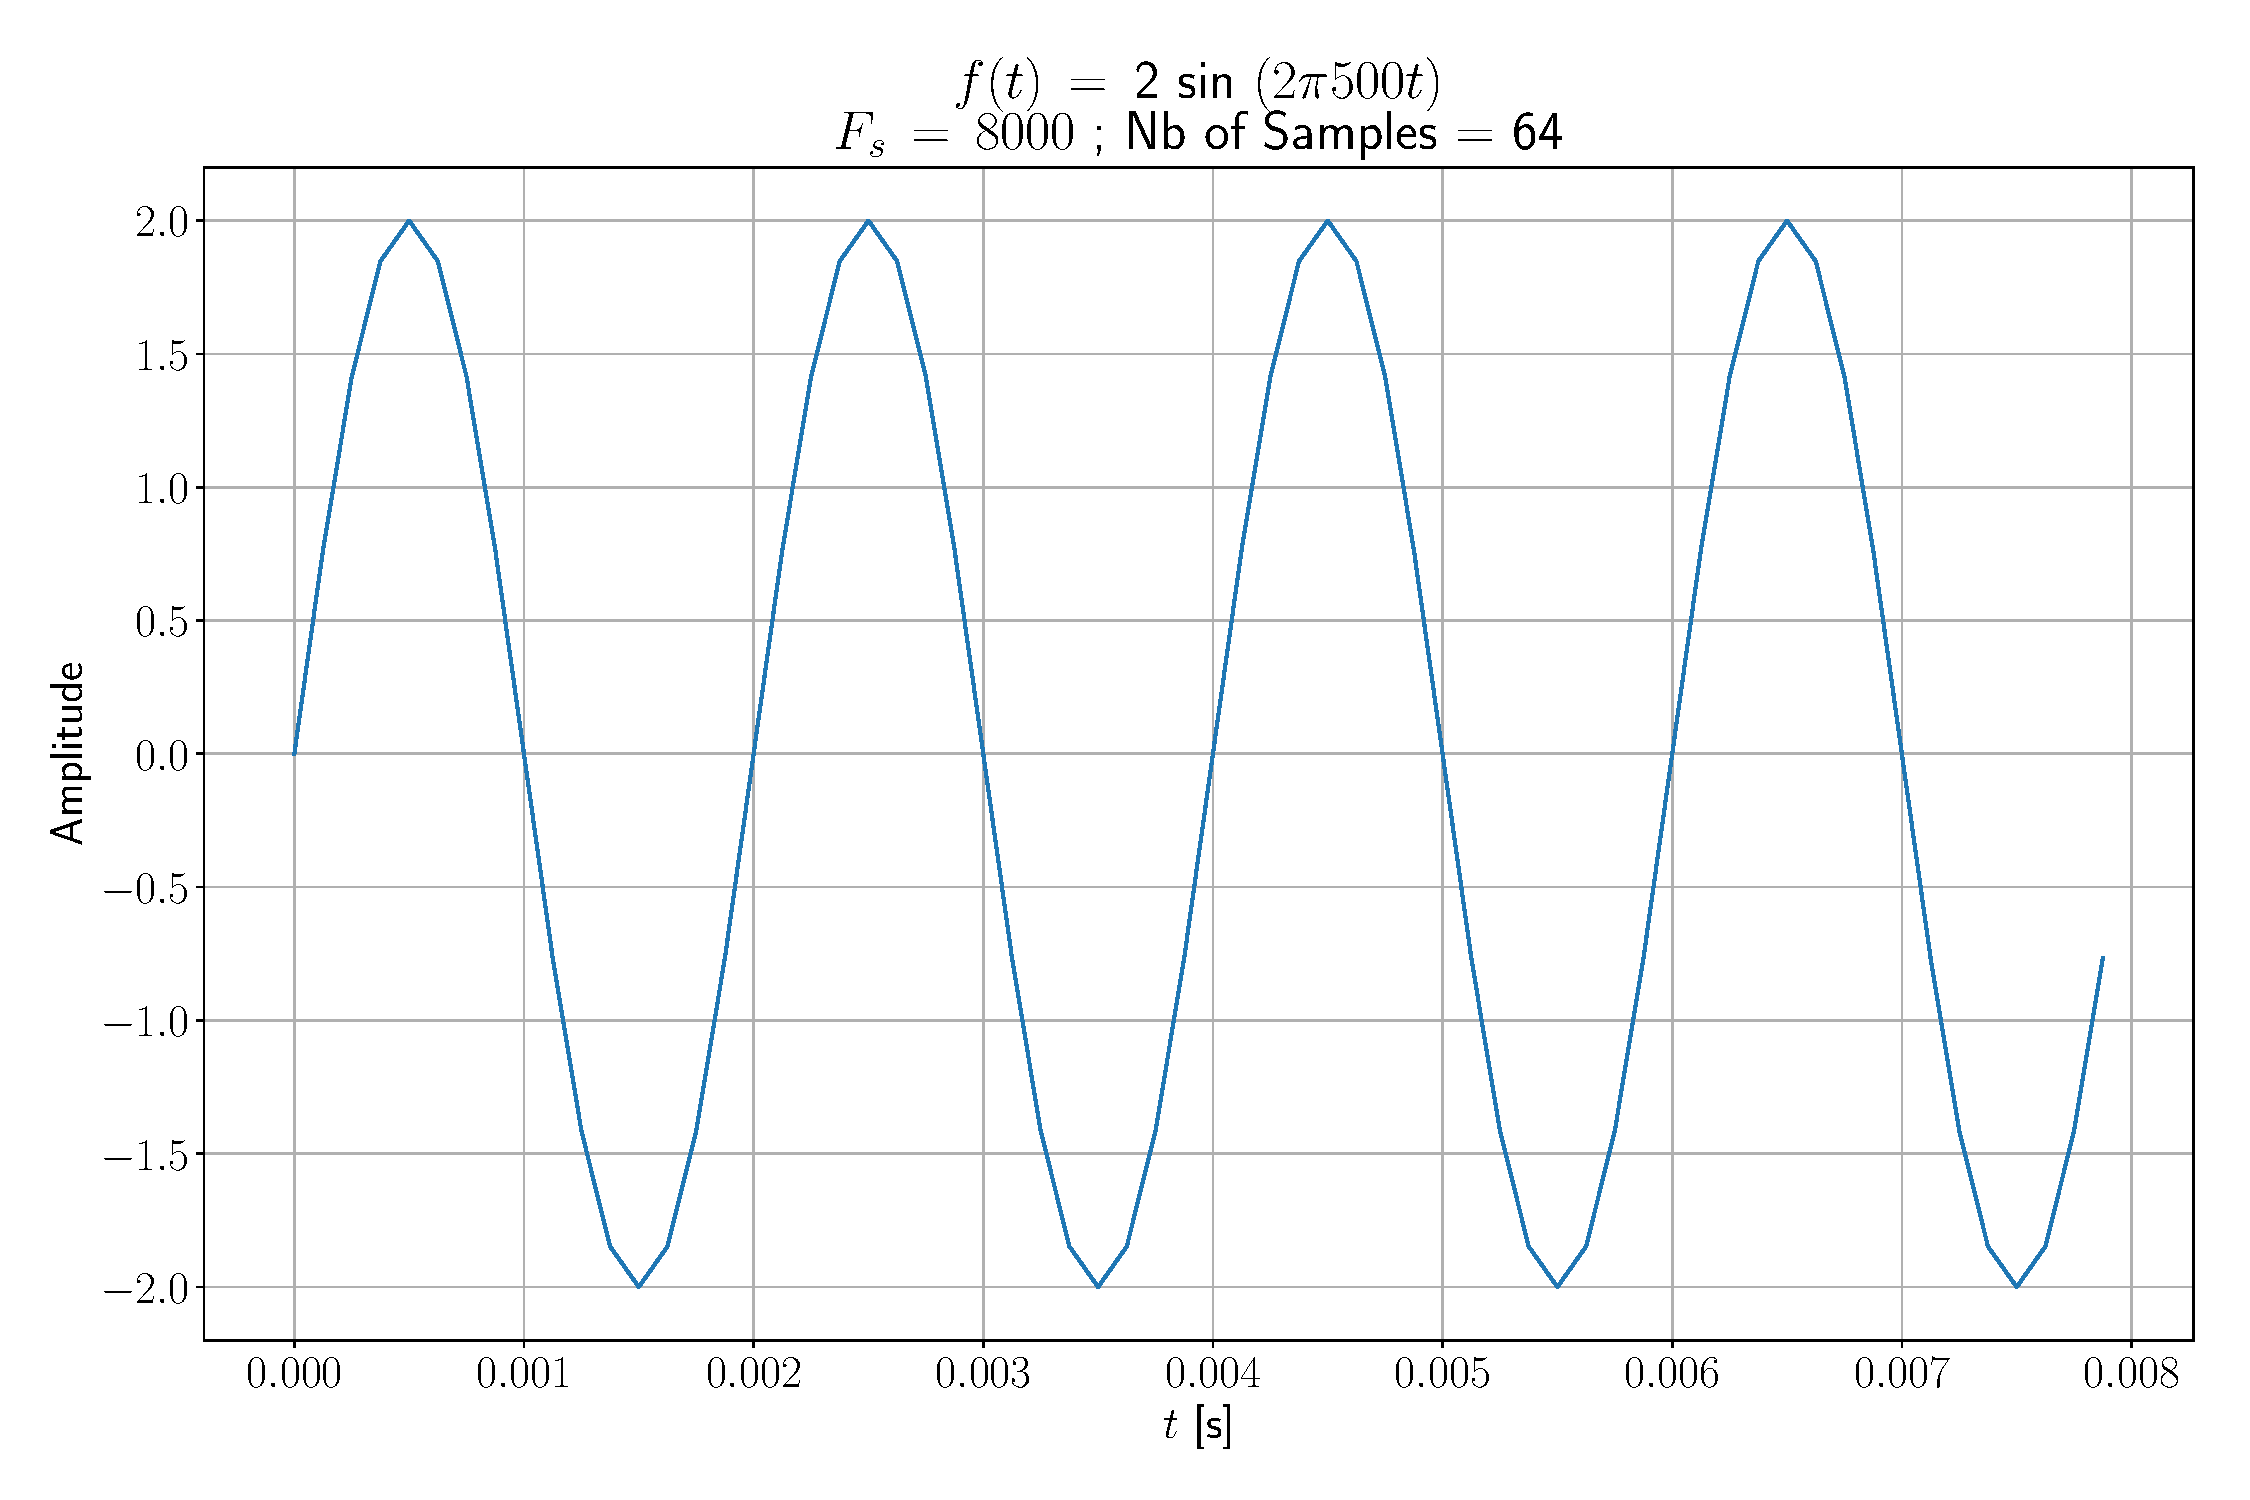
\includegraphics[width = 0.8\textwidth]{Figures/Simulation_Sampling_Frequency_Analysis/Spectral_Analysis_1_Sin_time_domain}
\caption{Time Domain Signal to be worked on}
\label{fig:Simulation_Sampling_Frequency_Analysis:Spectral_Analysis_1_Sin_time_domain}
\end{figure}


\begin{figure}[ht]
\centering
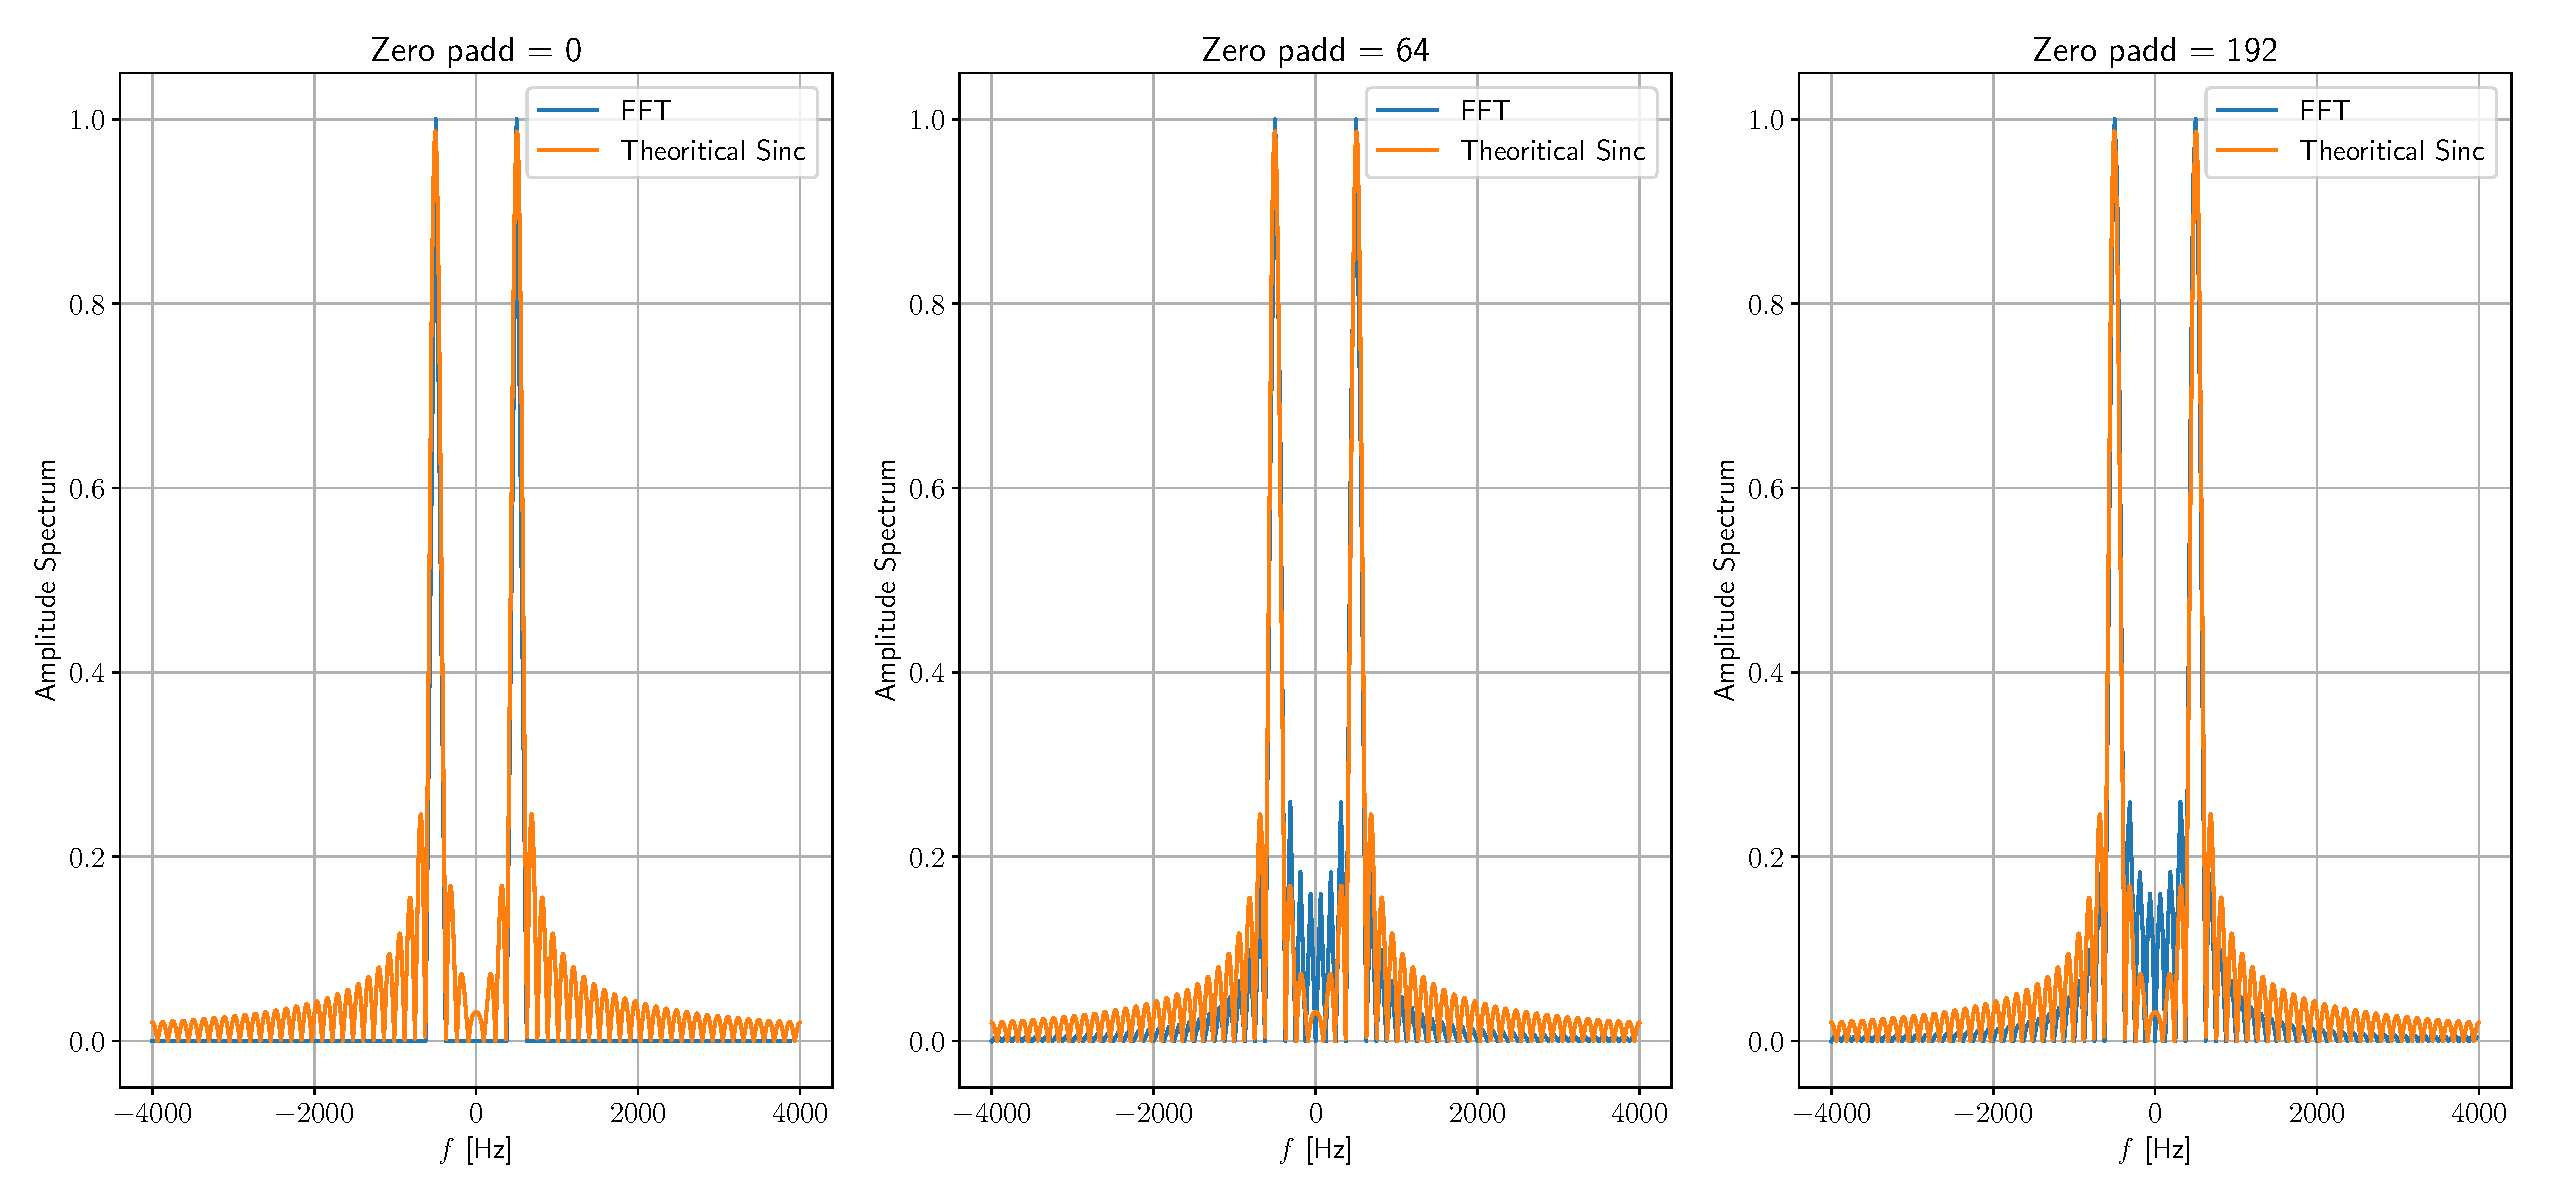
\includegraphics[width = 1\textwidth]{Figures/Simulation_Sampling_Frequency_Analysis/Spectral_Analysis_1_Sin}
\caption{Theoritical and Computed Spectrum using FFT}
\label{fig:Simulation_Sampling_Frequency_Analysis:Spectral_Analysis_1_Sin}
\end{figure}

\newpage

\begin{itemize}

\item If length of the FFT is the same of the length of the signal, no zero padding occur

\item If length of the FFT $>$ bigger then length of the signal, the signal will be padded with 0

	\begin{itemize}
	\item More \textcolor{red}{dense spectrum} is obtained $\leftrightarrow$ better displayed version $\leftrightarrow$ longer DFT sequence
	\end{itemize}

\end{itemize}


\end{frame}
